\noindent
\begin{minipage}[t]{0.485\textwidth}
\setlength{\parindent}{0pt}

\textbf{50.} Cho $g(x) = \operatorname{sgn}(\sin x)$.
\begin{enumerate}[label=\textnormal{(\alph*)}, nosep, leftmargin=1.5em]
    \item Tìm mỗi giới hạn sau hoặc giải thích vì sao giới hạn đó không tồn tại.
    \vspace{1pt}
    
    \begin{tabularx}{\linewidth}{@{}XXX@{}}
    (i) $\lim\limits_{x \to 0^+} g(x)$ & (ii) $\lim\limits_{x \to 0^-} g(x)$ & (iii) $\lim\limits_{x \to 0} g(x)$ \\[4pt]
    (iv) $\lim\limits_{x \to \pi^+} g(x)$ & (v) $\lim\limits_{x \to \pi^-} g(x)$ & (vi) $\lim\limits_{x \to \pi} g(x)$
    \end{tabularx}
    \vspace{1pt}
    \item Với những giá trị nào của $a$ thì $\lim\limits_{x \to a} g(x)$ không tồn tại?
    \item Vẽ đồ thị của hàm số $g$.
\end{enumerate}

\vspace{6pt}
\textbf{51.} Cho $g(x) = \dfrac{x^2 + x - 6}{|x - 2|}$.
\begin{enumerate}[label=\textnormal{(\alph*)}, nosep, leftmargin=1.5em]
    \item Tìm
    \vspace{1pt}
    
    \begin{tabularx}{\linewidth}{@{}XX@{}}
    (i) $\lim\limits_{x \to 2^+} g(x)$ & (ii) $\lim\limits_{x \to 2^-} g(x)$
    \end{tabularx}
    \vspace{1pt}
    \item Giới hạn $\lim\limits_{x \to 2} g(x)$ có tồn tại hay không?
    \item Vẽ đồ thị của hàm số $g$.
\end{enumerate}

\vspace{6pt}
\textbf{52.} Cho
\[
f(x) = \begin{cases}
x^2 + 1 & \text{nếu } x < 1 \\
(x - 2)^2 & \text{nếu } x \ge 1
\end{cases}
\]
\begin{enumerate}[label=\textnormal{(\alph*)}, nosep, leftmargin=1.5em]
    \item Tìm $\lim\limits_{x \to 1^-} f(x)$ và $\lim\limits_{x \to 1^+} f(x)$.
    \item Giới hạn $\lim\limits_{x \to 1} f(x)$ có tồn tại hay không?
    \item Vẽ đồ thị của hàm số $f$.
\end{enumerate}

\vspace{6pt}
\textbf{53.} Cho
\[
B(t) = \begin{cases}
4 - \frac{1}{2}t & \text{nếu } t < 2 \\
\sqrt{t + c} & \text{nếu } t \ge 2
\end{cases}
\]
Tìm giá trị của $c$ sao cho $\lim\limits_{t \to 2} B(t)$ tồn tại.

\vspace{6pt}
\textbf{54.} Cho
\[
g(x) = \begin{cases}
x & \text{nếu } x < 1 \\
3 & \text{nếu } x = 1 \\
2 - x^2 & \text{nếu } 1 < x \le 2 \\
x - 3 & \text{nếu } x > 2
\end{cases}
\]
\begin{enumerate}[label=\textnormal{(\alph*)}, nosep, leftmargin=1.5em]
    \item Tính mỗi giá trị sau, nếu tồn tại.
    \vspace{1pt}
    
    \begin{tabularx}{\linewidth}{@{}XXX@{}}
    (i) $\lim\limits_{x \to 1^-} g(x)$ & (ii) $\lim\limits_{x \to 1} g(x)$ & (iii) $g(1)$ \\[4pt]
    (iv) $\lim\limits_{x \to 2^-} g(x)$ & (v) $\lim\limits_{x \to 2^+} g(x)$ & (vi) $\lim\limits_{x \to 2} g(x)$
    \end{tabularx}
    \vspace{1pt}
    \item Vẽ đồ thị của hàm số $g$.
\end{enumerate}

\vspace{6pt}
\textbf{55.} \begin{enumerate}[label=\textnormal{(\alph*)}, nosep, leftmargin=1.5em]
    \item Nếu ký hiệu $\llbracket \; \rrbracket$ biểu thị hàm phần nguyên lớn nhất đã được định nghĩa trong Ví dụ 10, hãy tính
    \vspace{1pt}
    
    \begin{tabularx}{\linewidth}{@{}XXX@{}}
    (i) $\lim\limits_{x \to -2^+} \llbracket x \rrbracket$ & (ii) $\lim\limits_{x \to -2} \llbracket x \rrbracket$ & (iii) $\lim\limits_{x \to -2{,}4} \llbracket x \rrbracket$
    \end{tabularx}
    \vspace{1pt}
    \item Nếu $n$ là một số nguyên, hãy tính
    \vspace{1pt}
    
    \begin{tabularx}{\linewidth}{@{}XX@{}}
    (i) $\lim\limits_{x \to n^-} \llbracket x \rrbracket$ & (ii) $\lim\limits_{x \to n^+} \llbracket x \rrbracket$
    \end{tabularx}
    \vspace{1pt}
    \item Với những giá trị nào của $a$ thì $\lim\limits_{x \to a} \llbracket x \rrbracket$ tồn tại?
\end{enumerate}

\vspace{6pt}
\textbf{56.} Cho $f(x) = \llbracket \cos x \rrbracket$, $-\pi \le x \le \pi$.
\begin{enumerate}[label=\textnormal{(\alph*)}, nosep, leftmargin=1.5em]
    \item Vẽ đồ thị của hàm số $f$.
    \item Tính mỗi giới hạn sau, nếu tồn tại.
    \vspace{1pt}
    
    \begin{tabularx}{\linewidth}{@{}XX@{}}
    (i) $\lim\limits_{x \to 0} f(x)$ & (ii) $\lim\limits_{x \to (\pi/2)^-} f(x)$ \\[4pt]
    (iii) $\lim\limits_{x \to (\pi/2)^+} f(x)$ & (iv) $\lim\limits_{x \to \pi/2} f(x)$
    \end{tabularx}
    \vspace{1pt}
    \item Với những giá trị nào của $a$ thì $\lim\limits_{x \to a} f(x)$ tồn tại?
\end{enumerate}

\vspace{6pt}
\textbf{57.} Nếu $f(x) = \llbracket x \rrbracket + \llbracket -x \rrbracket$, hãy chứng minh rằng $\lim\limits_{x \to 2} f(x)$ tồn tại nhưng không bằng $f(2)$.

\end{minipage}%
\hfill
\begin{minipage}[t]{0.485\textwidth}
\setlength{\parindent}{0pt}

\textbf{58.} Trong thuyết tương đối, công thức co độ dài Lorentz
\[
L = L_0 \sqrt{1 - v^2/c^2}
\]
biểu thị chiều dài $L$ của một vật thể như một hàm số theo vận tốc $v$ của nó đối với một người quan sát, trong đó $L_0$ là chiều dài của vật thể khi đứng yên và $c$ là tốc độ ánh sáng. Hãy tìm $\lim\limits_{v \to c^-} L$ và giải thích ý nghĩa kết quả. Vì sao ở đây giới hạn bên trái lại cần thiết?

\vspace{5pt}
\textbf{59.} Nếu $p$ là một đa thức, hãy chứng minh rằng $\lim\limits_{x \to a} p(x) = p(a)$.

\vspace{5pt}
\textbf{60.} Nếu $r$ là một hàm phân thức hữu tỉ, hãy sử dụng Bài tập 59 để chứng minh rằng $\lim\limits_{x \to a} r(x) = r(a)$ với mọi số $a$ thuộc tập xác định của $r$.

\vspace{5pt}
\textbf{61.} Nếu $\lim\limits_{x \to 1} \dfrac{f(x) - 8}{x - 1} = 10$, hãy tìm $\lim\limits_{x \to 1} f(x)$.

\vspace{5pt}
\textbf{62.} Nếu $\lim\limits_{x \to 0} \dfrac{f(x)}{x^2} = 5$, hãy tìm các giới hạn sau.
\vspace{1pt}

\begin{tabularx}{\linewidth}{@{}XX@{}}
(a) $\lim\limits_{x \to 0} f(x)$ & (b) $\lim\limits_{x \to 0} \dfrac{f(x)}{x}$
\end{tabularx}

\vspace{5pt}
\textbf{63.} Cho hàm số
\[
f(x) = \begin{cases}
x^2 & \text{nếu } x \text{ là số hữu tỉ} \\
0 & \text{nếu } x \text{ là số vô tỉ}
\end{cases}
\]
hãy chứng minh rằng $\lim\limits_{x \to 0} f(x) = 0$.

\vspace{5pt}
\textbf{64.} Bằng cách đưa ra một ví dụ, hãy chỉ ra rằng $\lim\limits_{x \to a} [f(x) + g(x)]$ có thể tồn tại ngay cả khi cả $\lim\limits_{x \to a} f(x)$ lẫn $\lim\limits_{x \to a} g(x)$ đều không tồn tại.

\vspace{5pt}
\textbf{65.} Bằng cách đưa ra một ví dụ, hãy chỉ ra rằng $\lim\limits_{x \to a} [f(x)g(x)]$ có thể tồn tại ngay cả khi cả $\lim\limits_{x \to a} f(x)$ lẫn $\lim\limits_{x \to a} g(x)$ đều không tồn tại.

\vspace{5pt}
\textbf{66.} Tính $\lim\limits_{x \to 2} \dfrac{\sqrt{6 - x} - 2}{\sqrt{3 - x} - 1}$.

\vspace{5pt}
\textbf{67.} Có tồn tại số $a$ nào sao cho giới hạn
\[
\lim_{x \to -2} \frac{3x^2 + ax + a + 3}{x^2 + x - 2}
\]
tồn tại hay không? Nếu có, hãy tìm giá trị của $a$ và giá trị của giới hạn đó.

\vspace{5pt}
\textbf{68.} Hình vẽ bên dưới minh họa một đường tròn cố định $C_1$ có phương trình $(x - 1)^2 + y^2 = 1$ và một đường tròn đang co lại $C_2$ có bán kính $r$ và tâm tại gốc tọa độ. $P$ là điểm $(0, r)$, $Q$ là giao điểm phía trên của hai đường tròn, và $R$ là giao điểm của đường thẳng $PQ$ với trục $x$. Điều gì sẽ xảy ra với điểm $R$ khi đường tròn $C_2$ co lại dần, nghĩa là khi $r \to 0^+$?

\begin{center}
    \vspace{2pt}
    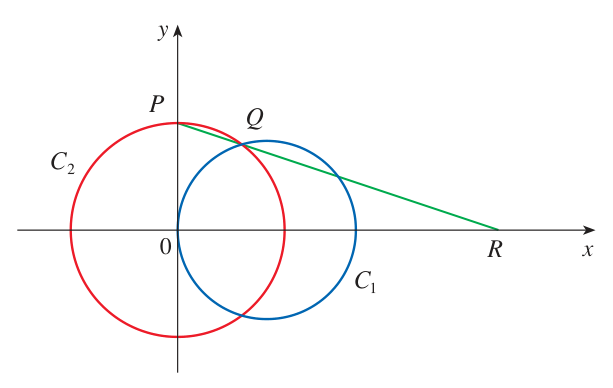
\includegraphics[width=0.72\linewidth]{images/p0139_fig1.png}
\end{center}

\end{minipage}
